\section{Grunnleggende notasjon og mengdelære}

\begin{definition}
    En \textit{mengde} er en samling objekter $S$ hvor vi kan for
    ethvert objekt $e$ vite om $e$ tilhører $S$, skrevet $e\in S$,
    eller ikke, skrevet $e\notin S$.

    Objektene som tilhører en mengde kalles \textit{elementene}
    i mengden.
\end{definition}

Vi noterer ofte en mengde med elementene den inneholder,
til eksempel skriver vi de naturlige tallene som
\[
    \mathbb N = \{0, 1, 2, \dots\}.
\]
\begin{example}
    De naturlige tallene $\mathbb N$, heltallene $\mathbb Z$,
    de rasjonale tallene $\mathbb Q$,
    de reelle tallene $\mathbb R$
    og de komplekse tallene $\mathbb C$ danner alle mengder.

    Det finnes en tom mengde $\emptyset = \{\}$,
    og vi kan lage mengder av mengder,
    slik som mengden av den tomme mengden $\{\emptyset\}\neq\emptyset$.
\end{example}

Det finnes også samlinger av objekter som ikke danner mengder.
\begin{example}
    Samlingen av alle mengder som ikke inneholder seg selv er ikke en mengde.
    Om vi snakker om samlinger som ikke er mengder fremhever vi ofte at de ikke
    er mengder ved å bruke for eksempel klammeparenteser,
    så denne samlingen kan skrives som
    \[
        \left[
            S
            \mid
            S\notin S
        \right]
    \]
\end{example}

\begin{remark}
    Et element er enten med i en mengde eller ikke
    -- det finnes ingen id\`e om flere av det samme elementet i en mengde.
    Altså om vi har $S = \{a,b\}$, men $a = b = 1$,
    så vil $S = \{1\}$.

    Om vi vil ha flere elementer, og samtidig bryr oss om rekkefølgen av elementer
    så bruker vi en \textit{tuppel} $(a,b)$,
    så om $a = b = 1$ har vi $(a, b) = (1,1) \neq (1)$,
    men for $a\neq b$ har vi $(a, b)\neq (b, a)$.
\end{remark}

\begin{definition}
    En \textit{avbildning} $f\colon A\to B$ mellom to mengder er en
    regel som for ethvert element $a\in A$ assosierer et element
    $b = f(a)\in A$.

    Vi kaller $A$ \textit{definisjonsmengden} til $f$
    og $B$ \textit{verdimengden}.
    Vi definerer også en delmengde av $B$
    \[
        \im f = \{b\in B\mid \mbox{det finnes $a\in A$ slik at } f(a) = b\}
        \subset B
    \]
    som vi kaller \textit{bildet} av $f$.

    Vi tegner ofte opp avbildninger som piler,
    så om vi har flere mengder $A, B, C$, men flere avbildninger
    $f\colon A\to B, g\colon A\to C, h\colon B\to C$
    imellom seg kan vi tegne det opp som
    \[
        \begin{tikzcd}
            A
            \ar{rr}{f}
            \ar{rd}{g}
            &&
            B
            \ar{ld}{h}
            \\
            &
            C.
        \end{tikzcd}
    \]
\end{definition}

For ethvert element $a\in A$ finnes det bare \`en verdi for $f(a)\in B$.
Derimot kan flere verdier $a, a^\prime$ avbilde på samme verdi
$f(a) = f(a^\prime)$.

\begin{example}
    For enhver mengde $A$ finnes det en naturlig avbildning
    $\id_A\colon A\to A$ som sender hvert element $a\in A$
    på seg selv $a\mapsto a$
\end{example}

\begin{remark}
    Merk at for enhver mengde $A$ så finnes det
    nøyaktig en avbildning $\emptyset \to A$,
    men det finnes ingen avbildning $A\to \emptyset$ med mindre $A = \emptyset$.
\end{remark}

\begin{example}
    Om vi har to avbildninger $A\xrightarrow{f} B\xrightarrow{g} C$
    kan vi lage en ny avbildning $g\circ f\colon A\to C$
    ved å sende $g\circ f(a) = g(f(a))$ for alle $a\in A$.
\end{example}

\begin{definition}
    En avbildning $f\colon A\to B$ er \textit{injektiv} om for alle $a,b\in A$ med $a\neq b$
    så er $f(a)\neq f(b)$.
    Om $f$ er injektiv skriver vi ofte pilen som $f\colon A\hookrightarrow B$
    og sier at $f$ er en \textit{inklusjon}.

    Avbildningen er \textit{surjektiv} om for alle $b\in B$ så finnes en $a\in A$
    slik at $f(a) = b$.
    Om $f$ er surjektiv skriver vi noen ganger pilen som
    $f\colon A\twoheadrightarrow B$ og sier at $f$ er en \textit{surjeksjon}.

    Om $f$ er både injektiv og surjektiv sier vi den er \textit{bijektiv}
    og sier $f$ er en \textit{bijeksjon}.
\end{definition}

\begin{lemma}\label{thm:set-inverse-function}
    Om $f\colon A\to B$ er en bijeksjon så finnes en unik avbildning
    $g\colon B\to A$ slik at $f\circ g = \id_B$ og $g\circ f = \id_A$,
    dvs.
    $f(g(b)) = b$ for alle $b\in B$ og $g(f(a)) = a$ for alle $a\in A$.
    Vi kaller $g$ \textit{inversavbildningen} til $f$ og skriver $f^{-1} = g$.
\end{lemma}
\begin{proof}
    Definer en regel $g\colon B\to A$ som for hver $b\in B$ finner en $a\in A$
    slik at $f(a) = b$.
    En slik $a$ finnes alltid for enhver $b$ siden $f$ er surjektiv.

    La $g^\prime$ være en annen funksjon konstruert på samme måte,
    det vil si $g^\prime$ tilfredsstiller $f(g^\prime(b)) = b$ for alle $b\in B$.
    Men $f(g(b)) = b = f(g^\prime(b))$ og $f$ er injektiv, så $g(b) = g^\prime(b)$
    for alle $b\in B$, så $g = g^\prime$.
\end{proof}

\begin{example}
    For en mengde $A$ er $\id_A$ en bijeksjon,
    og inversavbildningen er avbildningen selv $\id_A = \id_A^{-1}$.
\end{example}

\begin{example}
    Vi kan ta \textit{snitt} og \textit{union} av mengder for å skape nye mengder.
    Snittet av to mengder $A,B$ er mengden av elementer som ligger i både $A$ og $B$
    \[
        A\cap B = \{ e\mid e\in A\mbox{ og } e\in B\},
    \]
    mens unionen er mengden av elementer i enten $A$ eller $B$
    \[
        A\cup B = \{ e\mid e\in A\mbox{ eller } e\in B\}.
    \]

    Når vi tar snitt og union følger det med naturlige inklusjoner
    \[\begin{tikzcd}
        A\cap B
        \rar[hook]
        \dar[hook]
        & B
        \dar[hook]
        \\
        A
        \rar[hook]
        &
        A\cup B
    \end{tikzcd}\].
    Disse er så naturlige at vi benevner dem som $A\cap B\subset A,B\subset A\cup B$
    utenfor diagrammer, altså er snittet $A\cap B$
    en \textit{delmengde} av $A$ (og $B$),
    og $A$ (og $B$) er en delmengde av $A\cup B$.
\end{example}

\begin{example}
    Vi har $\{1,\dots,10\}\cap \{5,\dots,15\} = \{5, 6, 7, 8, 9, 10\}$,
    og $\{1,\dots, 10,\}\cup \{5,\dots, 15\} = \{1,\dots, 15\}$.
\end{example}

\begin{definition}
    Vi kan ta \textit{komplementet} av to mengder $A, B$
    \[
        A\setminus B = \{ a\in A\mid a\notin B\} \subset A.
    \]
\end{definition}

\begin{example}
    Vi kan ta produktet av to mengder $A, B$.
    Dette er mengden
    \[
        A\times B = \{
            (a,b)\mid a\in A,\, b\in B
        \}.
    \]
    Her følger også med noen avbildninger
    \[\begin{tikzcd}
        A
        \rar[<-]{p}
        &
        A\times B
        \rar{q}
        &
        B
    \end{tikzcd}\]
    hvor $p\colon (a,b)\mapsto a$ og $q\colon (a,b)\mapsto b$ er
    projeksjonene til første og andre element henholdsvis.
\end{example}

\begin{example}
    Produktmengden til $\{0,\dots,9\}$ med seg selv består av hunder elementer,
    og vi har en bijeksjon $\{0,\dots,9\}\times\{0,\dots,9\}\to \{0,\dots,99\}$
    gitt ved $(n, m)\mapsto 10n + m$.
\end{example}

\begin{definition}
    Vi kan snakke om størrelsen på en mengde $A$ -- altså \textit{kardinaliteten}
    til mengden, som vi benevner $|A|$ eller $\# A$.
    Om $A$ inneholder et endelig antall elementer,
    så er $\# A$ antall elementer i $A$.
    Om $A$ ikke er endelig kan vi fortsatt snakke om kardinaliteten til $A$,
    og vi kan sammenligne kardinaliteter,
    for om det finnes en inklusjon $A\hookrightarrow B$
    kan vi si $\# A\leq \# B$,
    og om det finnes en bijeksjon så har vi $\# A = \# B$.
\end{definition}

\begin{example}
    Vi har
    \[
        \mathbb N
        \subset \mathbb Z
        \subset \mathbb Q
        \subset \mathbb R
        \subset \mathbb C
    \]
    så åpenbart har vi
    \[
        \#\mathbb N
        \leq \#\mathbb Z
        \leq \#\mathbb Q
        \leq \#\mathbb R
        \leq \#\mathbb C,
    \]
    men det viser seg at
    \[
        \#\mathbb N
        = \#\mathbb Z
        = \#\mathbb Q
        < \#\mathbb R
        = \#\mathbb C.
    \]
    Merk at $\mathbb Z$ og $\mathbb R$ har forskjellig kardinalitet,
    men begge er uendelige.
    Vi benevner den første uendeligheten med $\aleph_0 = \#\mathbb Z$,
    og den sistnevnte som $\aleph_1 = \#\mathbb R$.
\end{example}

\begin{example}
    La $A, B$ være to mengder.
    Vi kan lage mengden av alle avbildninger fra $A$ til $B$
    \[
        \mathrm{Map}(A,B) = \{f\colon A\to B\}.
    \]
    Vi sier to avbildninger $f,g\colon A\to B$
    er like om $f(a) = g(a)$ for alle $a\in A$.
\end{example}

\subsubsection*{Oppgaver}

\begin{enumerate}
    \item Vis at om $f\colon A\hookrightarrow B$ er en injeksjon
        så finnes en $g\colon B\twoheadrightarrow A$ slik at
        $g\circ f = \id_A$.
        Er den unik?
    \item La $A\xrightarrow{f} B\xrightarrow{g} C$ være to avbildninger.
        \begin{enumerate}
            \item
                Anta $g\circ f$ er surjektiv.
                Vis at da må $f$ være surjektiv.
            \item
                Anta $g\circ f$ er injektiv.
                Vis at da må $f$ være injektiv.
            \item
                Om $g\circ f$ er en bijeksjon, må $f$ eller $g$ være en bijeksjon?
        \end{enumerate}
    \item La $U$ være en mengde, og $A, B\subset U$ to delmengder.
        Vis identiteten
        \[
            U\setminus(A\cap B) = (U\setminus A)\cup (U\setminus B).
        \]
    \item La $A, B$ være to endelige mengder, og la $n = \# A$ og $m=\# B$,
        vis at da er $\# \mathrm{Map}(A,B) = m^n$.
        Dette motiverer hvorfor flere forfattere velger å skrive
        $\mathrm{Map}(A,B) = B^A$.
    \item La $\mathrm{Bij}(A)$ benevne mengden av bijeksjoner $s\colon A\to A$,
        og la $f\colon A\to B$ være en bijeksjon.
        Vis at avbildningen $\tilde f\colon \mathrm{Bij}(A)\to \mathrm{Bij}(B)$
        gitt ved $s\mapsto f\circ s\circ f^{-1}$ er en bijeksjon.
\end{enumerate}
Mengdeteoretisk definerer vi ofte en avbildning $A\to B$ som en samling data
$(A, B, \Gamma)$ med $\Gamma\subset A\times B$ slik at for alle $a\in A$
så finnes en unik $b\in B$ slik at $(a,b)\in \Gamma$.
Denne delmengden $\Gamma$ kalles \textit{grafen} til funksjonen,
for om vi skal gi den tilhørende ``regelen'' $f$ får vi $f(a) = b$
for alle $(a,b)\in \Gamma$.

\begin{remark}
    Merk at for en $A\to B$ er både $A$ og $B$ del av
    dataen, så for to avbildninger $f, g$ med definisjonsmengde
    $A$ og samme graf $\Gamma_f = \Gamma_g$ så kan de være forskjellige
    om de har forskjellige verdimengder $B_f, B_g$,
    til eksempel om $B_g\subsetneq B_f$.
\end{remark}
\begin{example}
    La $f\colon \mathbb Z\to \mathbb Z$ og
    $g\colon \mathbb Z\to 2\mathbb Z$
    hvor
    \[
        2\mathbb Z = \{2n \mid n\in \mathbb Z\}\subset \mathbb Z.
    \]
    Både $f$ og $g$ er gitt ved $f(n) = g(n) = 4n$ for alle $n\in \mathbb Z$,
    så de har samme bilde i $\im f = \im g\subset\mathbb Z$,
    men de har forskjellig verdimengde, så $f\neq g$.
\end{example}
\begin{enumerate}[resume]
    \item
        \begin{enumerate}
            \item Hva betyr det for $\Gamma$ at $f$ er injektiv?
            \item Hva betyr det for $\Gamma$ at $f$ er surjektiv?
            \item Kan du bevise \cref{thm:set-inverse-function} på en annen
                måte ved å bruke denne nye definisjonen av en avbildning?
        \end{enumerate}
\end{enumerate}

\begin{figure}[htb]
    \centering
    \begin{subfigure}[b]{.3\textwidth}
        \centering
        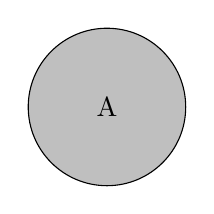
\begin{tikzpicture}
            \draw[fill=lightgray] (0,0) circle (1);
            \draw (0,0) node {A};
        \end{tikzpicture}
        \caption{En mengde $A$}
    \end{subfigure}
    \begin{subfigure}[b]{.3\textwidth}
        \centering
        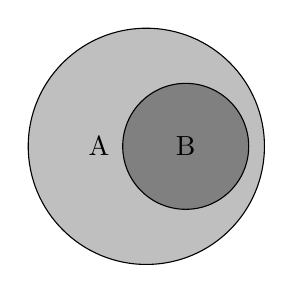
\begin{tikzpicture}
            \draw[fill=lightgray] (0,0) circle (1.5);
            \draw[fill=gray] (.5,0) circle (.8);
            \draw (-.6,0) node {A};
            \draw (.5, 0) node {B};
        \end{tikzpicture}
        \caption{$B\subset A$}
    \end{subfigure}
    \begin{subfigure}[b]{.3\textwidth}
        \centering
        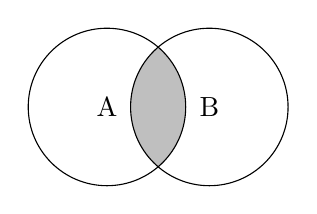
\begin{tikzpicture}
            \coordinate (a) at (0,0);
            \coordinate (b) at (1.3, 0);
            \begin{scope}
                \clip (b) circle (1);
                \fill[lightgray] (a) circle (1);
            \end{scope}
            \draw (a) node{A} circle(1);
            \draw (b) node{B} circle(1);
        \end{tikzpicture}
        \caption{$A\cap B$}
    \end{subfigure}
    \begin{subfigure}[b]{.3\textwidth}
        \centering
        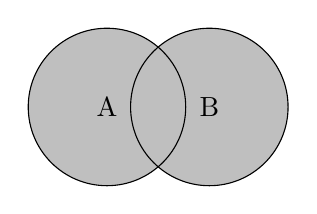
\begin{tikzpicture}
            \coordinate (a) at (0,0);
            \coordinate (b) at (1.3, 0);
            \fill[lightgray] (a) circle (1)
                (b) circle (1);
            \draw (a) node{A} circle(1);
            \draw (b) node{B} circle(1);
        \end{tikzpicture}
        \caption{$A\cup B$}
    \end{subfigure}
    \begin{subfigure}[b]{.3\textwidth}
        \centering
        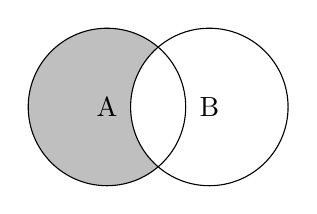
\begin{tikzpicture}
            \coordinate (a) at (0,0);
            \coordinate (b) at (1.3, 0);
            \begin{scope}[even odd rule]
                \clip (a) circle (1) (b) circle (1);
                \fill[lightgray] (a) circle (1);
            \end{scope}
            \draw (a) node{A} circle(1);
            \draw (b) node{B} circle(1);
        \end{tikzpicture}
        \caption{$A\setminus B$}
    \end{subfigure}
    \begin{subfigure}[b]{.38\textwidth}
        \centering
        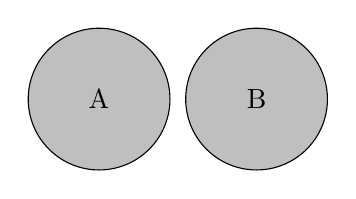
\begin{tikzpicture}
            \coordinate (a) at (0,0);
            \coordinate (b) at (2, 0);
            \draw[fill=lightgray] (a) node{A} circle(.9);
            \draw[fill=lightgray] (b) node{B} circle(.9);
        \end{tikzpicture}
        \caption{$A\cap B=\emptyset$}
    \end{subfigure}
    \caption{Konsepter om mengder.}
\end{figure}

\begin{figure}
    \centering
    \begin{subfigure}[b]{.49\textwidth}
        \centering
        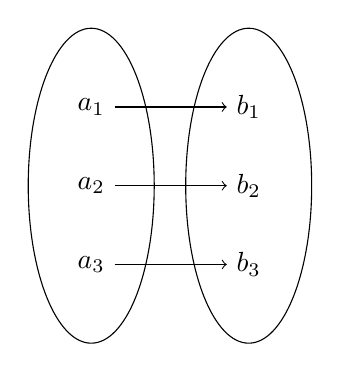
\begin{tikzpicture}
            \begin{scope}
                \draw (0,0) node (a1) {$a_1$}
                    ++(0,-1) node (a2) {$a_2$}
                    ++(0,-1) node (a3) {$a_3$};
                \draw (a2) ellipse (.8 and 2);
            \end{scope}
            \begin{scope}[xshift=2cm]
                \draw (0,0) node (b1) {$b_1$}
                    ++(0,-1) node (b2) {$b_2$}
                    ++(0,-1) node (b3) {$b_3$};
                \draw (b2) ellipse (.8 and 2);
            \end{scope}
            \draw[->] (a1) -- (b1);
            \draw[->] (a2) -- (b2);
            \draw[->] (a3) -- (b3);
        \end{tikzpicture}
        \caption{En bijeksjon.}
    \end{subfigure}
    \begin{subfigure}[b]{.49\textwidth}
        \centering
        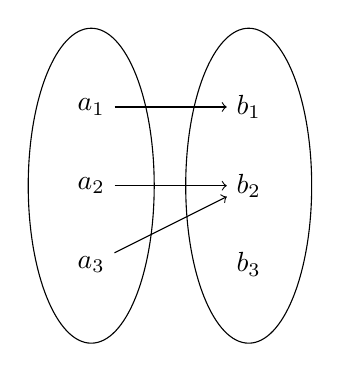
\begin{tikzpicture}
            \begin{scope}
                \draw (0,0) node (a1) {$a_1$}
                    ++(0,-1) node (a2) {$a_2$}
                    ++(0,-1) node (a3) {$a_3$};
                \draw (a2) ellipse (.8 and 2);
            \end{scope}
            \begin{scope}[xshift=2cm]
                \draw (0,0) node (b1) {$b_1$}
                    ++(0,-1) node (b2) {$b_2$}
                    ++(0,-1) node (b3) {$b_3$};
                \draw (b2) ellipse (.8 and 2);
            \end{scope}
            \draw[->] (a1) -- (b1);
            \draw[->] (a2) -- (b2);
            \draw[->] (a3) -- (b2);
        \end{tikzpicture}
        \caption{Hverken en injeksjon eller surjeksjon.}
    \end{subfigure}
    \begin{subfigure}[b]{.49\textwidth}
        \centering
        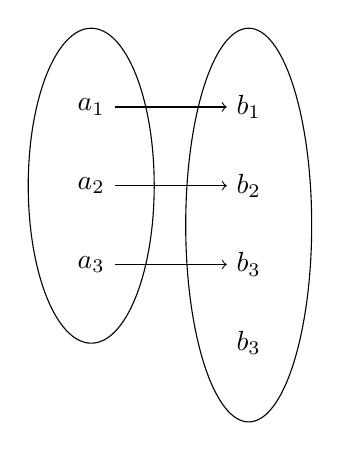
\begin{tikzpicture}
            \begin{scope}
                \draw (0,0) node (a1) {$a_1$}
                    ++(0,-1) node (a2) {$a_2$}
                    ++(0,-1) node (a3) {$a_3$};
                \draw (a2) ellipse (.8 and 2);
            \end{scope}
            \begin{scope}[xshift=2cm]
                \draw (0,0) node (b1) {$b_1$}
                    ++(0,-1) node (b2) {$b_2$}
                    ++(0,-1) node (b3) {$b_3$}
                    ++(0,-1) node (b4) {$b_3$};
                \path (b2) -- (b3) coordinate[midway] (c){};
                \draw (c) ellipse (.8 and 2.5);
            \end{scope}
            \draw[->] (a1) -- (b1);
            \draw[->] (a2) -- (b2);
            \draw[->] (a3) -- (b3);
        \end{tikzpicture}
        \caption{En injeksjon.}
    \end{subfigure}
    \begin{subfigure}[b]{.49\textwidth}
        \centering
        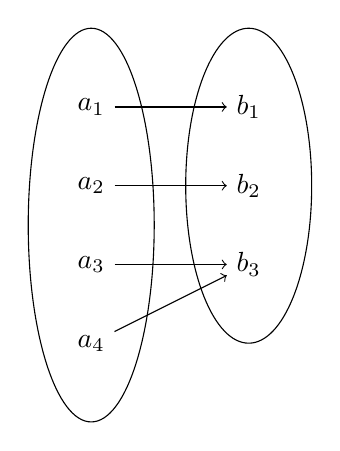
\begin{tikzpicture}
            \begin{scope}
                \draw (0,0) node (a1) {$a_1$}
                    ++(0,-1) node (a2) {$a_2$}
                    ++(0,-1) node (a3) {$a_3$}
                    ++(0,-1) node (a4) {$a_4$};
                \path (a2) -- (a3) coordinate[midway] (c);
                \draw (c) ellipse (.8 and 2.5);
            \end{scope}
            \begin{scope}[xshift=2cm]
                \draw (0,0) node (b1) {$b_1$}
                    ++(0,-1) node (b2) {$b_2$}
                    ++(0,-1) node (b3) {$b_3$};
                \draw (b2) ellipse (.8 and 2);
            \end{scope}
            \draw[->] (a1) -- (b1);
            \draw[->] (a2) -- (b2);
            \draw[->] (a3) -- (b3);
            \draw[->] (a4) -- (b3);
        \end{tikzpicture}
        \caption{En surjeksjon.}
    \end{subfigure}
    \caption{Konsepter om avbildninger.}
\end{figure}

\subsection{Mengdelære i kryptografi}

Mengdelære er et veldig fundamentalt område innen matematikken,
men enda kan vi bruke noen av disse primitive redskapene til å si noe om
kryptografiske metoder.

Vi har sett fire kategorier av kryptografiske metoder,
nemlig
\begin{itemize}
    \item hashing,
    \item symmetrisk kryptering,
    \item asymmetrisk kryptering, og
    \item nøkkelutveksling.
\end{itemize}
Disse kan alle beskrives som avbildninger,
og vi kan allerede si at disse avbildningene må tilfredsstille visse egenskaper,
men først må vi definere mengdene disse avbildningene avbilder imellom.

Ofte er det tre mengder vi har i tankene,
\begin{itemize}
    \item $\mathscr M$ -- mengden av meldinger som Alice og Bob kan tenke seg å
        sende.
        Dette kan være mengden av alle tekster som kan tenkes og skrives,
        eller det kan være en forhåndsbestemt mengde av bare et fåtall uttrykk,
        slik som $\{\mathrm{Ja}, \mathrm{Nei}\}$.
    \item $\mathscr K$ -- mengden av nøkler som kan velges av Alice og Bob.
    \item $\mathscr C$ -- mengden av mulige chiffertekster.
\end{itemize}

\subsubsection{Hash-funksjoner}
En hashfunksjon i generell forstand er bare en avbildning $h\colon \mathscr M\to \mathscr C$.
Ofte ønsker vi noe som heter en \textit{perfekt} hash som vil si at om vi har to forskjellige
meldinger $m\neq m^\prime\in \mathscr M$ så hashes meldingene til forskjellige
chiffertekster $h(m)\neq h(m^\prime)\in \mathscr C$.
I kryptografi er det ofte tilstrekkelig at det ikke er ``for mange'' meldinger
som har samme chiffertekst,
men vi stiller ofte andre strenge krav til hvordan chifferteksten skal
skille seg mellom ulike meldinger.

\subsubsection{Symmetrisk kryptering}
En symmetrisk krypteringsalgoritme er to avbildninger
$f\colon \mathscr M\times \mathscr K\to \mathscr C$
og $g\colon \mathscr C\times \mathscr Kt\to \mathscr M$
slik at for alle $m\in \mathscr M$ og $k\in \mathscr K$
har vi $g(f(m, k),k) = m$.
Om vi velger en fast nøkkel $k\in \mathscr K$ kan vi definere
to nye funksjoner
\[
    f_k\colon \begin{cases}
        \mathscr M\to \mathscr C
        \\
        m\mapsto f(m, k)
    \end{cases}
\]
og
\[
    g_k\colon \begin{cases}
        \mathscr C\to \mathscr M
        \\
        c\mapsto g(c, k),
    \end{cases}
\]
så $g_k\circ f_k = \id_{\mathscr M}$.
Spesielt betyr dette at $f_k$ må være injektiv,
og $g_k$ blir dermed surjektiv.

\subsubsection{Asymmetrisk kryptering}
En asymmetrisk algoritme er nesten  det samme,
men nå kan vi tenke oss at $f$ og $g$ bruker
bare delvis informasjon om nøkkelen.
Nå kan vi tenke oss en nøkkel $k\in\mathscr K$ som et par
$k = (k_a, k_b)$ hvor $k_a\in \mathscr K_a$ velges blant
en mengde private nøkler,
og $k_b\in \mathscr K_b$ velges blant en mengde offentlige nøkler,
så $\mathscr K\subset \mathscr K_a\times\mathscr K_b$.

Nå blir de to funksjonene gitt ved
\[\begin{aligned}
    f&\colon\mathscr M\times \mathscr K_a\to \mathscr C\\
    g&\colon\mathscr C\times \mathscr K_b\to \mathscr M
\end{aligned}\]
slik at $g_{k_b}\circ f_{k_a} = \id_{\mathscr M}$.
Det som er viktig her er at $(k_a, k_b)$ alltid opptrer i par
slik at for hver $k_a\in\mathscr K_a$ finnes en unik $k_b\in\mathscr K_b$
slik at $g_{k_b}\circ f_{k_a} = \id_{\mathscr M}$ og visa versa.
Det følger at vi har en bijeksjon $\mathscr K_a\to\mathscr K_b$
som for hver private nøkkel gir den tilhørende offentlige nøkkelen,
men denne bijeksjonen må være umulig å beregne for at algoritmen skal være sikker.
Merk at $\mathcal K\subset \mathcal K_a\times \mathcal K_b$ er grafen til denne bijeksjonen.
For at algoritmen skal være brukbar må det derimot være mulig å trekke tilfeldige
nøkkelpar $(k_a, k_b)$ fra $\mathcal K$.

\subsubsection{Nøkkelutveksling}
I klassisk Diffie-Hellman er algoritmen for Alice og Bob identisk,
så vi har to funksjoner
\[\begin{aligned}
    f&\colon \mathscr K\times\mathscr K\to \mathscr K
    \\
    g&\colon \mathscr K\to \mathscr K
\end{aligned}\]
slik at om Alice velger en nøkkel $k_a$ og Bob en nøkkel $k_b$
har vi $f(k_a, g(k_b)) = f(k_b, g(k_a))$.
Her er $g(k_a$ Alice sin offentlige nøkkel som hun deler med Bob,
og $g(k_b)$ er Bob sin offentlige nøkkel som han deler med Alice.
For algoritmens sikkerhet er det viktig at man ikke kan regne ut
$k$ fra $g(k)$, og at gitt $g(k_a)$ og $g(k_b)$
kan vi ikke regne ut $f(k_a, g(k_b))$.
